\documentclass[12pt]{article}
\usepackage[a4paper, total={6in, 8in}]{geometry}
\usepackage[english,polish]{babel}
\usepackage[T1]{fontenc}
\usepackage{minted}
\usepackage{listings}
\usepackage{geometry}
\usepackage{graphicx}
\graphicspath{ {./} }
\setlength{\parindent}{0pt}

\title{Podstawy kryptografii \\ \large Zastosowanie kryptografii asymetrycznej - protokół Diffiego-Hellmana}
\author{Adam Olech}


\begin{document}
\maketitle

\tableofcontents
\newpage

\section{Wyniki eksperymentu z Cryptoolem}

\subsection{Moduł liczby pierwszej 47}

W tym przegiegu użyto małej liczby pierwszej 47 oraz liczby generatora 29.

\begin{center}
	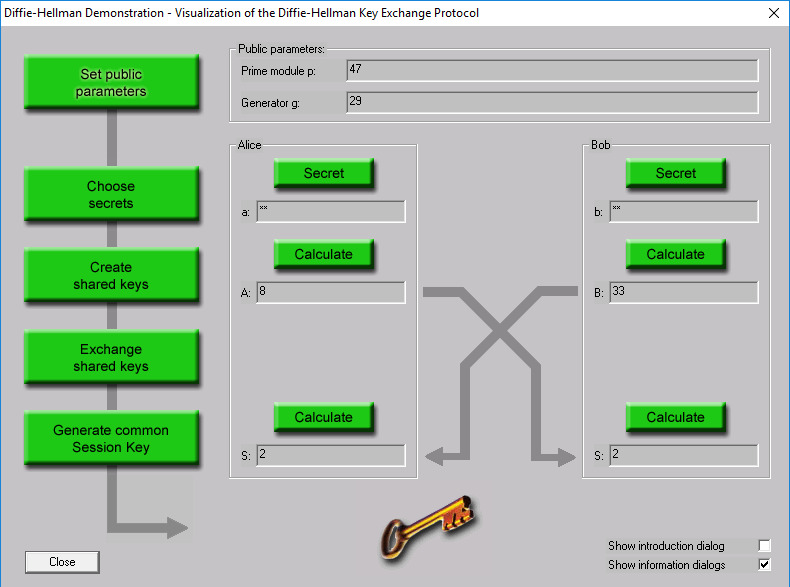
\includegraphics[scale=0.4]{4-cryptool-1}
\end{center}

Alice wybrała swoją utajnioną liczbę $a$ o wartości $16$.
Bob natomiast ustalił analogicznie liczbę $b$ o wartości $31$.

Jeśli któraś z liczb $a$ i $b$ byłaby większa lub równa od modułu $p$, to należałoby je zredukować.
W tym przypadku nie było to konieczne.

Na podstawie uprzednio wybranych liczb, Alice i Bob tworzą liczby, które wymienią miedzy sobą.

W tym przypadku, te liczby to $8$ i $33$ kolejno.

Na podstawie wymienionych miedzy sobą liczb, Alice i Bob w niezależny sposób są w stanie wyliczyć klucz sesyjny (obojgu powinien wyjść ten sam).

W przypadku tego eksperymentu, uzyskaną wartością była liczba $2$.

\newpage

\subsection{Moduł dużej liczby pierwszej}

W kolejnym przebiegu jako moduł $p$ użyto następującej dużej liczby pierwszej odkrytej przez Édouarda Lucasa w 1876 roku:

\begin{equation}
	170141183460469231731687303715884105727
\end{equation}

Liczba ta ma 39 cyfr.

\begin{center}
	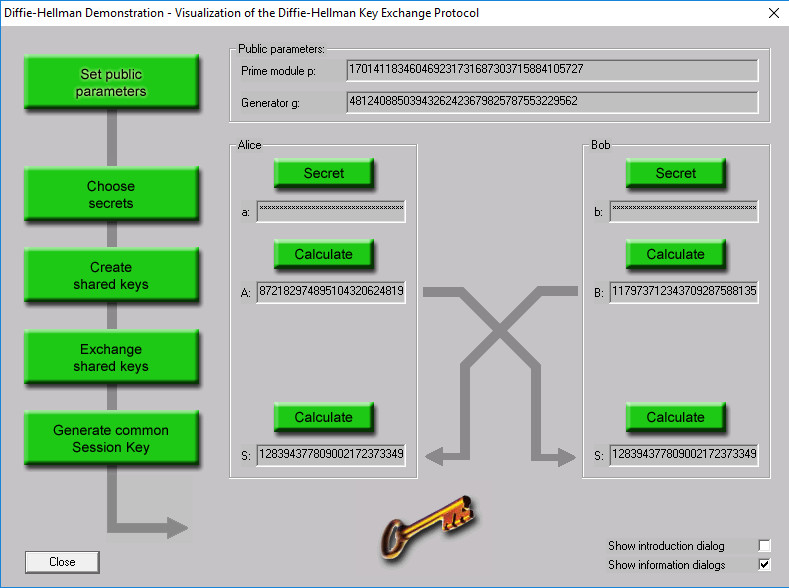
\includegraphics[scale=0.4]{4-cryptool-2}
\end{center}

W wyniku działania programu uzyskano następujące wartości:
\begin{itemize}
	\item \textbf{g}: 48124088503943262423679825787553229562
	\item \textbf{a}: 65963387705922719929071035848729932502
	\item \textbf{b}: 83098014163721153996622330633805783168
	\item \textbf{A}: 87218297489510432062481913308967573137
	\item \textbf{B}: 117973712343709287588135853382854744351
	\item \textbf{SA}: 128394377809002172373349938856329444803
	\item \textbf{SB}: 128394377809002172373349938856329444803
\end{itemize}

Obie wartości końcowe są takie same.

\section{Opis protokołu Diffiego-Hellmana}

Na początku komunikacji Alice i Bob wspólnie i jawnie uzgadniają, że będą używać danej liczby $p$ oraz $g$ (warto tutaj wspomnieć, że w przypadku biblioteki \textit{OpenSSL} ten parametr domyślnie przyjmuje wartość $2$).
Ważne jest, by przy każdej kolejnej sesji używali innego zestawu liczb.

\begin{figure}[h!]
	\begin{center}
		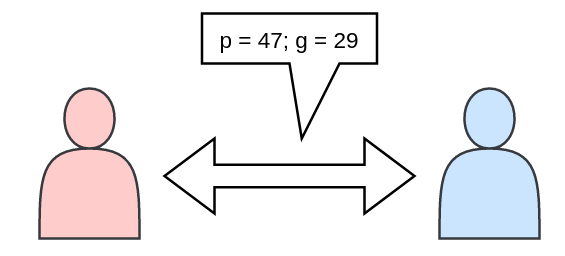
\includegraphics[scale=0.3]{4-dh-diagram-1}
	\end{center}
	\caption{Uzgodnienie początkowych parametrów}
\end{figure}

Następnie, każde z nich z osobna wybiera tajną liczbę i przesyła do siebie nawzajem resztę z dzielnia liczby $g$ podniesionej do potęgi tajnej liczby przez liczbę $p$.

\begin{figure}[h!]
	\begin{center}
		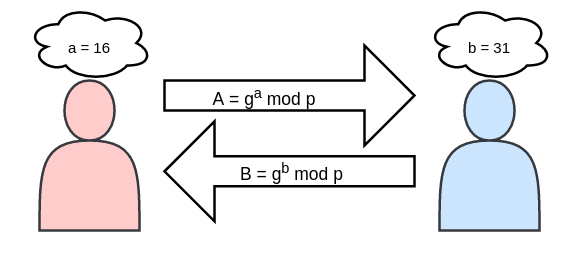
\includegraphics[scale=0.3]{4-dh-diagram-2}
	\end{center}
	\caption{Wysłanie liczb A i B}
\end{figure}

Na sam koniec, Alice i Bob oddzielnie wyliczają resztę z dzielnie otrzymanej liczby podniesionej do potęgi swojej tajnej liczby przez liczbę $p$.
Wbrew naiwnej intuicji, pomimo różnych parametrów, oboje uzyskują tę samą liczbę.

\begin{figure}[h!]
	\begin{center}
		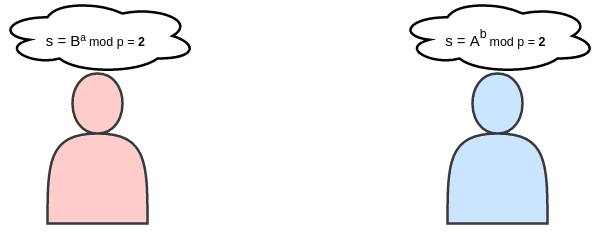
\includegraphics[scale=0.3]{4-dh-diagram-3}
	\end{center}
	\caption{Wysłanie liczb A i B}
\end{figure}
\end{document}
